\section{司法権の違いからくるリスク}
\subsection{概要}
クラウドの司法権の違いからくるリスクとして,国の法律の違いから,データの保存場所によっては,自国の秘密データを開示されてしまったり,不正にデータをとられてしまったりということが考えられる.例えば,企業の顧客データが複数の司法管轄域に保存されている場合,司法の整備が不十分な国などでは,襲撃されたり,強制開示を求められ,顧客データが流出してしまう恐れがある.そのため,データを安全に保存することが求められている.その例として,シーランド公国という自称国家をデータの避難場所にしようという動きがあった.さらに,e-discovery法という法律によって実際に日本の企業が他国の法律からデータを抜き取られた例から司法権の違いによるリスクについて考える.

\subsection{シーランド公国におけるデータヘイブン計画}
\subsubsection{シーランド公国}
シーランド公国\cite{sealand}とは,イギリス南東部のサフォーク州の10km沖合いに浮かぶ構造物を領土と主張する自称国家.しかし,2014年現在,国連に加盟する193か国及びバチカン市国の計194か国の中でシーランド公国を国家承認している国はない.シーランド公国を利用した様々な事業が考えられてきたが,そのほとんどが失敗に終わっている.今現在はオンラインショップで公国の貴族の証である爵位の販売を行ったりしている.シーランド公国の歴史は以下の通りである.
\begin{verbatim}
1942年 イギリス軍が北海の沖合約10kmの地点に海上要塞を建設 
1945年 終戦でイギリス軍が海上要塞を放棄
1967年9月2日 ロイ・ベイツ氏が海上要塞を占拠.シーランド公国の独立を宣言
\end{verbatim}

\begin{figure}[h!]
\begin{center}
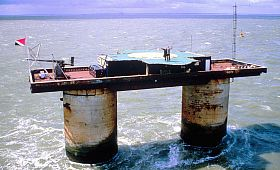
\includegraphics[scale=0.5]{shima}
\caption{シーランド公国}
\end{center}
\end{figure}

\subsubsection{データヘイブン計画}
米国のサイファーパンクたちが,シーランド公国で,秘密データや問題データを安全に保管する場所を求める人々のためのバーチャル・ヘイブン(避難地)を提供しようとしている動きがあった.ヘイブンコー社は、世界で最も強力なプライバシー保護と法的保護を提供することができるといい,ヘイブンコー社を作るために,創立者たちはシーランド公国のロイ・ベーツ公と契約を結んだが,各国政府からの批判も受けている\cite{sealand}.データ・ヘイブンとは,データの待避所として扱われるコンピュータもしくはコンピュータネットワークの一種である.それが保持するデータは,技術的手段(暗号化)とその立地条件によって政府の干渉から守られる.具体的な立地条件とは,設置された国においてデータの利用を制約する法律が無い・もしくは法律が僅かしか強制力を持たず、犯罪人引渡し条約が無いことである.ヘイブンコー(集中型)とフリーネット(分散型)が今日的なデータ・ヘイブンの2つの典型例である\cite{dataheaven}.シーランド公国は自称国家であるため,ここにデータを保存すれば,他国政府等からの干渉から守られると考えられた.


\subsection{e-discovery法}
\subsubsection{e-discovery法とは}
e-discovery法とは,電子情報の証拠開示手続き民事訴訟の当事者に,関連した電子メールや図面など,内部の電子データ開示を求める2006年に施行された米国の制度.データを提示できないと制裁を受ける.米国で訴訟を起こされれば,日本の本社やデータセンターなどにある電子証拠もすべて開示対象になる\cite{ediscovery}.
\subsubsection{e-discovery法により影響を受けた日本企業の事例}
\begin{itemize}
\item 東芝\\
2007年に,通信・ネットワーク業界大手の米国ジュニパーネットワークス社が,ノート型PCのメモリコントローラを巡る特許侵害で東芝社を訴えた判例.東芝側は,当該ソースコードの開示義務を知りながら,開示を意図的に回避する決断をした.その後のヒアリングで,東芝は自社が所有・管理する全ての関連証拠を開示したとし,未開示のソースコードは第三者の手元にあり開示することができないと主張したが,ソースコード設計者のデポジションにより覆され,実際は東芝がこのソースコードを所有していることが判明した.最終的に東芝は開示に応じたが,裁判に不利な制裁を受けた\cite{ediscoveryblog}.
\item 武田薬品工業\\
武田薬品工業株式会社が,イスラエルを本拠とするジェネリックメーカーのTevaPharmaceuticalをデラウェア州連邦地方裁判所に提訴。裁判所は,原告の武田製薬工業に18年分の電子データを開示し,  その費用の2割を負担するよう申し渡した\cite{ediscoveryblog}.
\item ブラザー社\\
2007年に,インクカートリッジの設計と関連する取引方法を巡ってkandelに起こされた訴訟では,ブラザー社が原告に誤って秘匿特権文書を開示.裁判所は,被告が当該文書の開示を防ぐための適切な措置および,開示後に文書回収のための適切な措置を迅速に講じたため,秘匿特権文書の返還を認めた\cite{ediscoveryblog}.
\item 日産ノースアメリカ\\
香港に本社を置くJohnsonElectronics社の不良部品が元となり,一部車種のリコールを強いられたとして、日産ノースアメリカが損害賠償を求めている事例.これまで,日産は179万ページの文書ならびに,本件の当事者ではない日本本社からも8万4千ページの文書を開示している.今回,被告が新たに求めた開示に対し,当該データへのアクセスには過度の負担が伴うとして,日産が保護命令を申請した.裁判所は,原告の保護命令申し立ては認められないとの判決を下した\cite{ediscoveryblog}.
\item トヨタ\\
2010年アメリカで,トヨタ車の運転中に発生した急加速事故についての調査や訴訟が行われた.この事故に関するトヨタの社内資料の翻訳に携わった日英翻訳者が,トヨタの内部資料を公表した.ディスカバディー資料の情報流出が問題となっている\cite{ediscoveryblog}.
\end{itemize}


\subsubsection{対策}
企業が訴えられることは日常的にあるわけではないが,企業側は常に,「このデータを削除したら業務に支障がでないか」ということを意識して,不要な情報の削除を行っていく必要がある.そのようなリスク管理が求められる.
